% !TEX root = ../thesis.tex

\chapter{关键技术介绍}

一个直播系统的构成需要有视频的编解码技术、以及流媒体传输协议等技术支持,在基于AV1的低延迟直播系统搭建的过程中,面对着流媒体传输协议的选择,我们需要根据直播系统的业务特点与需求出发,选择最合适的直播协议来契合整个系统。

\section{视频编码标准}

本章将对视频编码进行简要介绍,并对比分析常用视频编码标准的编码效率与专利费用情况。并对AV1视频编码标准进行介绍,包括AV1的编码框架与编码工具、AV1的研究进展、AV1的多层预测帧结构,以及与下文对AV1进行RTP封装相关的AV1开放比特流单元(OBU)。
\subsection{视频编码概述}

视频编码技术利用视频在时间和空间维度上的冗余性,对原始的视频序列进行压缩,减小视频文件的码率,以便于存储和传输。视频编码技术发展中,有两类重要的编码技术:预测编码与变换编码。预测编码通过分析临近像素在时间与空间上的相关性,利用已经编码的像素对需要编码的像素进行预测,只需对预测误差进行编码,因为残差信息相比原始像素的数据量更小,可以获得编码增益。变换编码对空间域下的图像进行某种变换,得到变换域中的数据表达,改变数据分布以减少有效数据量。将两种编码技术结合使用的方式称作混合编码,使用混合编码可以获得比单独使用一种编码技术更高的压缩效率。

为了进一步提高压缩效率,在混合编码框架中加入了针对运动目标的运动估计和运动补偿机制。通过运动估计(Motion Estimation, ME)得到物体的运动矢量(Motion Vector, MV),根据运动矢量计算前后帧的运动物体对应点的差值称作运动补偿(Motion Compensation, MC)。通过这种机制可以减少帧间预测的误差,提高帧间预测压缩效率。

量化(Quantization)和熵编码(Entropy Coding)是预测、变换后的两个重要处理技术。变换后,数据在变换域中呈不均匀分布,能量主要集中在直流与低频区域,因此采用非均匀量化,对低频区域执行细量化,对高频区域执行粗量化,可以减小量化误差。量化是数据损失的过程,引入了失真,提升了压缩效率。熵编码表示一个符号的码字长度随符号出现概率变化,为高概率符号分配较短码字、为低概率符号分配较长码字,熵编码可以提供比等长编码更高的编码效率。

视频编码的性能取决于编码码率、失真、计算复杂度三者的折中选择。考虑如何在限制的码率条件下,为编码选择合适的模式与参数以最小化编码失真的技术称为率失真优化\cite{sullivanRatedistortionOptimizationVideo1998}(Rate Distortion Optimization, RDO)。

以上介绍了视频编码中的核心技术,包括预测、变换编码、量化、率失真优化、熵编码等,实际应用中,组合运用上述技术以实现视频的高效压缩。
\subsection{视频编码标准对比\label{sec:codec-comparison}}

视频编码标准指的是规定了所用的视频编码技术集合、相对应的编码结果比特流及编解码规范的标准。视频编码标准主要由ITU与ISO/IEC两大组织制定。ITU制定的视频编码标准为H.26X系列,广泛应用于基于网络传输的视频通信,ISO/IEC的动态图像专家组(Moving Picture Experts Group, MPEG)制定的MPEG系列视频编码标准主要应用于视频存储等。两大组织的合作已经产生了H.264/AVC、H.265/HEVC,再下一代的标准H.266/VVC也正在开发中。近年来一些新的视频编码标准进入市场,有VP8、VP9、Daala、Thor等,以及由提出这些标准的公司组成的开放媒体联盟(AOMedia)开发的下一代视频编码标准:AV1。

不同视频编码标准的差异在于其编码效率、解码效率、计算复杂度、及专利费用等。不同视频编码标准的性能对比在操作上是非常困难的\cite{laudeComprehensiveVideoCodec2019}:
% 有点偏题啊
\begin{enumerate} [label=\arabic*)]
  \item 视频编码标准仅规定了所用技术与比特流格式,能产生符合标准的比特流的实际的编码器实现可以有很大差异,例如参考编码器与用于生产环境的编码器相比往往在质量上稍好,但在速度上慢的多;
  \item 不同编码器的预设配置及配置API不同,导致难以将两个不同编码标准的编码器调整到同等配置;
  \item 在不同测试序列的表现不同,一种视频编码标准或一个编码器实现可能在一类视频序列上表现好,但在另一些序列表现差,往往难以选择对所有编码器都公平的测试序列;
\end{enumerate}

\begin{table}[!hpt]
  \renewcommand{\arraystretch}{0.9}
  \caption{常用视频编码标准对比}
  \label{tab:codec}
  \centering
  \begin{tabular}{cccc}
  	\toprule
  	  Codec    & Year & 编码效率  & 专利费用 \\ \midrule
  	H.264/AVC  & 2003 & 50\%  &  \$  \\ %50.7\%  37.6\%  0  -3.8\%  -27.5\%
  	   VP9     & 2013 & 37\%  & free \\
  	H.265/HEVC & 2013 &   /   & \$\$ \\
  	   AV1     & 2018 & -10\% & free \\
  	H.266/VVC  & TBD  & -30\% & \$\$ \\ \bottomrule
  \end{tabular}
\end{table}

由于本文的重点不是对比不同视频编码标准,因此在此根据文献\cite{groisCodingEfficiencyComparison2016, akyaziComparisonCompressionEfficiency2018a, zhangComparingVVCHEVC2020}列出对当前常用的几个编码标准的简单比较。如表\ref{tab:codec}所示,MPEG/ITU系列视频编码标准约每十年更新一代,AOM系列的视频编码标准约每五年更新一代,每一代视频编码标准对比前一代标准在复杂度与编码效率均有提升。AOM系列的标准与MPEG/ITU系列相比的优势在于其免版税的特性。

综合对比后选择AV1作为直播系统的编码标准,有以下考虑:
\begin{enumerate} [label=\arabic*)]
  \item AV1的免版税特性,相比HEVC的版税及专利问题有巨大优势;
  \item AV1是当前最新一代的编码标准,编码效率高;
  \item AV1设计旨在用于互联网上的视频传输,适合视频直播的应用场景。
\end{enumerate}

\subsection{AV1视频编码标准}

AOMedia Video 1\cite{rivazAV1BitstreamDecoding2019}(AV1)是一种开放的,免版税的视频编码格式,旨在用于互联网上的视频传输,取代Google的VP9并与H.265/HEVC竞争。AV1由开放媒体联盟AOMedia开发,该联盟的成员有半导体行业公司,视频点播提供商,视频内容提供商,软件开发公司和Web浏览器供应商等。

\begin{figure}[!htp]
	\centering
	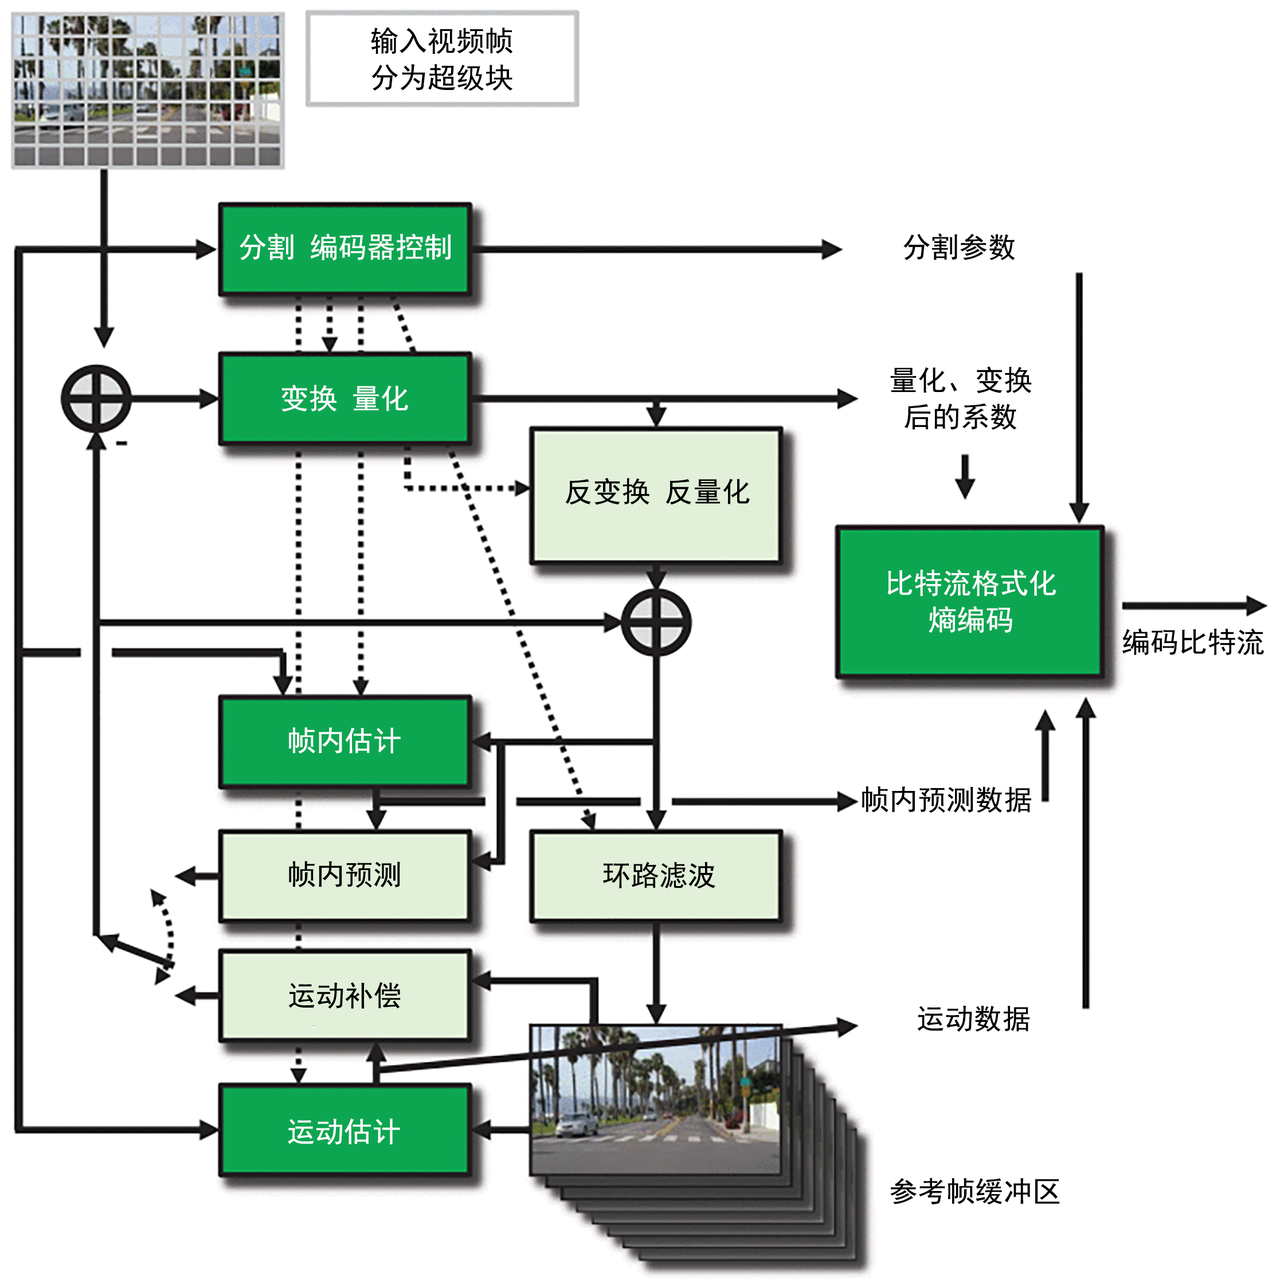
\includegraphics[width=0.7\linewidth]{av1_structure.png}
	\caption{AV1编码框架\cite{trowAV1ImplementationPerformance2020}}
	\label{fig:av1-structure}
\end{figure}

AOMedia的成员组成了完整的产业链,共同创建的AV1更是具有开放、免版税的特性,与需要缴纳专利费的HEVC不同,有利于AV1在开源项目中的使用,构建良好的生态系统。在功能上,AV1专为实时高质量视频分发(尤其是WebRTC)和更高的分辨率,更宽的色域,更高的帧速率,在各种带宽上对现代设备的可伸缩性设计,而不是当前主流视频格式H.264的典型使用场景。

如图\ref{fig:av1-structure},AV1使用经典的混合视频编码框架,包含许多先进的编码工具\cite{chenOverviewCoreCoding2018},包括更多样的分块方案,更多的帧内预测选项,从亮度预测色度\cite{trudeauPredictingChromaLuma2018a},针对屏幕内容的调色盘模式、帧内块复制\cite{liIntraBlockCopy2018},更多的参考帧\cite{linEfficientAV1Video2018},更灵活的运动向量估计以及其他帧间预测工具。环路滤波和后处理使用了约束方向增强滤波器(CDEF)\cite{midtskogenAv1ConstrainedDirectional2018}和环路滤波帧超分辨率\cite{joshiInloopFrameSuperresolution2019}、胶片颗粒合成\cite{norkinFilmGrainSynthesis2018}等工具。这些先进的编码工具使得AV1可以达到更高的编码效率。

AV1最近的研究进展有基于JND的RDO感知优化\cite{zhuJNDbasedPerceptualRate2019}、用机器学习的方法加速AV1编码\cite{suMachineLearningAccelerated2019, dingCNNbasedInloopFiltering2019},快速算法,包括快速帧间预测决策树算法\cite{kimFastInterPredictionBased2019}块划分快速算法\cite{guoFastBlockStructure2018}、模式选择快速算法\cite{jeongFastIntraMode2019}、变换模式选择的快速算法优化\cite{luEfficientRatedistortionApproximation2018}等,对AV1编码的研究正在稳步发展。
\subsubsection{AV1多层预测帧结构}


AV1使用了许多先进的编码工具,值得一提的是AV1更更强大的帧间编码器。AV1对参考帧和运动矢量进行了扩展,将参考帧数从3个扩展到7个。除了VP9的最近过去(LAST)帧,遥远过去(GOLDEN)帧和临时过滤未来(ALTREF)帧之外,还添加了两个最近过去帧(LAST2和LAST3)和两个将来帧(BWDREF和ALTREF2)\cite{linEfficientAV1Video2018}。

\begin{figure}[!htp]
	\centering
	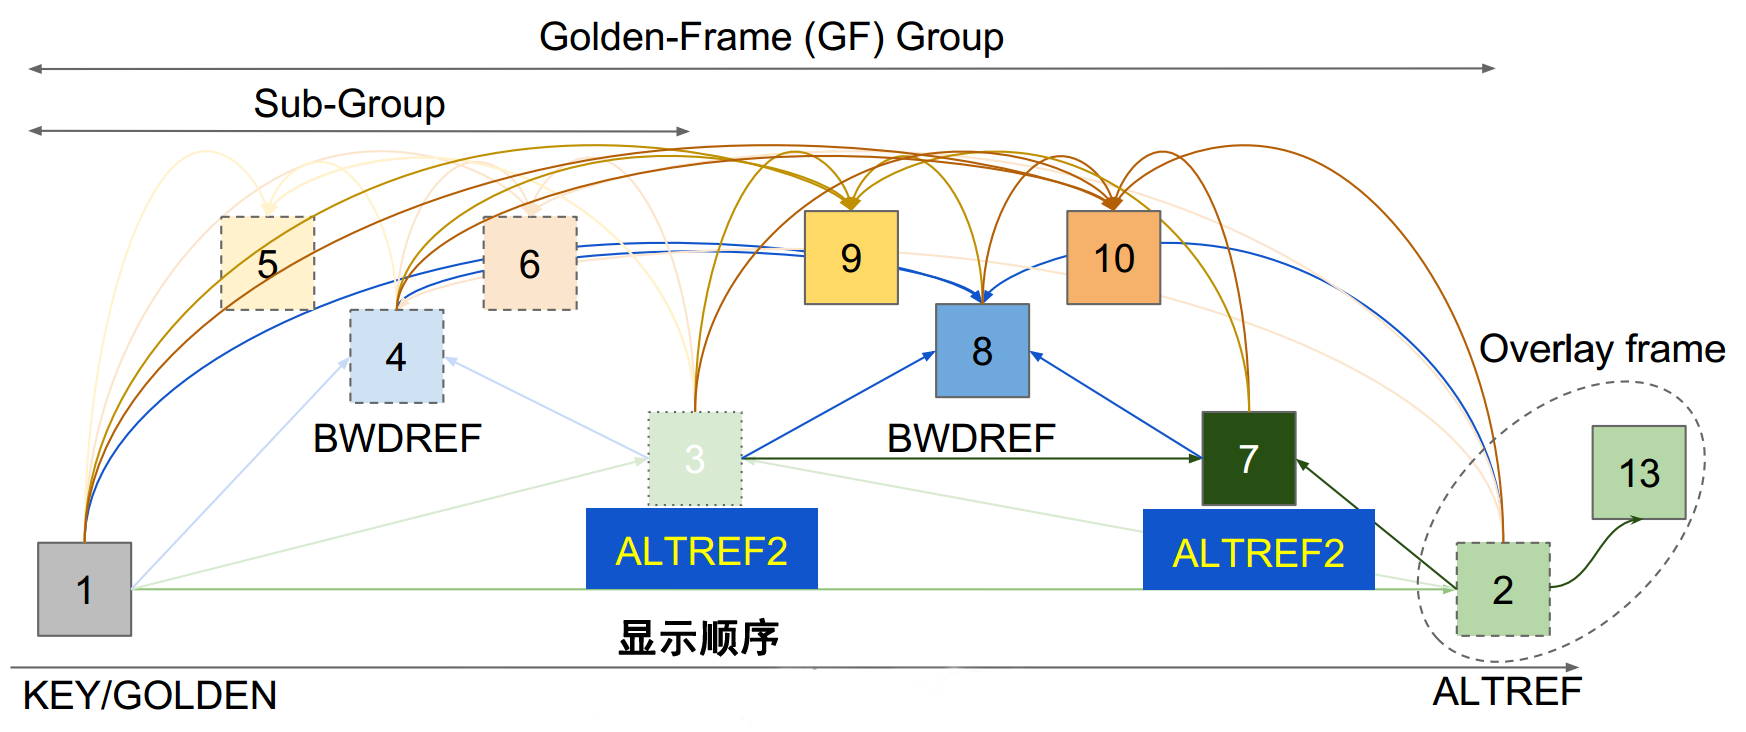
\includegraphics[width=0.8\linewidth]{av1-multi-layer-structure.png}
	\caption{AV1黄金帧组的多层预测框架\cite{chenOverviewCoreCoding2018}}
	\label{fig:av1-multi-layer-structure}
\end{figure}

图\ref{fig:av1-multi-layer-structure}展示了黄金帧组的多层预测结构\cite{chenOverviewCoreCoding2018},其中自适应数量的帧共享相同的GOLDEN和ALTREF帧。 BWDREF是直接编码的超前帧,无需应用时间滤波,适合用作相对较短距离的后向参考。ALTREF2用作GOLDEN和ALTREF之间的帧的将来参考。所有新参考帧都可以通过单个预测模式选择,也可以组合成对以形成复合模式。AV1提供了丰富的参考帧对集合,同时提供了双向复合预测和单向复合预测,因此可以用更自适应和最优的方式对具有动态时间相关性特征的各种视频进行编码。

\subsubsection{AV1开放比特流单元}
本文不涉及过多的AV1编码工具原理,但是涉及AV1码流的相关知识。AV1码流被封装成“开放比特流单元(OBU)”这种低开销的比特流格式。每个OBU由一个\texttt{obu\_header}和相对应类型的obu载荷构成。AV1的OBU类型如表\ref{tab:obutype}所示,每个编码序列有一个\texttt{OBU\_SEQUENCE\_HEADER}包含该码流的序列编码信息;\texttt{OBU\_TEMPORAL\_DELIMITER}表示时间分割符,包含空载荷;\texttt{OBU\_FRAME\_HEADER}包含了编码的一帧的头信息;\texttt{OBU\_TILE\_GROUP}包含一个Tile内部的各个superblock分割类型、预测变换类型以及参数等解码需要的信息;\texttt{OBU\_FRAME}包含一个\texttt{OBU\_FRAME\_HEADER}和一个\texttt{OBU\_TILE\_GROUP}。在后续RTP封装的时候,由于RTP封装的payload大小限制,这些OBU会根据规则分割装入不同的RTP包。

\begin{table}[!hpt]
    \renewcommand{\arraystretch}{0.8}
    \caption{AV1比特流标准:obu\_type}
    \label{tab:obutype}
    \centering
    \begin{tabular}{cc} \toprule
      obu\_type & Name of obu\_type\\ \midrule
      0    & \texttt{Reserved}  \\
      1    & \texttt{OBU\_SEQUENCE\_HEADER}     \\
      2    & \texttt{OBU\_TEMPORAL\_DELIMITER}   \\
      3    & \texttt{OBU\_FRAME\_HEADER}   \\
      4    & \texttt{OBU\_TILE\_GROUP}     \\
      5    & \texttt{OBU\_METADATA}     \\
      6    & \texttt{OBU\_FRAME}     \\
      7    & \texttt{OBU\_REDUNDANT\_FRAME\_HEADER}     \\
      8    & \texttt{OBU\_TILE\_LIST}     \\
      9-14 & \texttt{Reserved}     \\
      15   & \texttt{OBU\_PADDING}     \\ \bottomrule
    \end{tabular}
  \end{table}


\section{流媒体协议与封装协议选择}

协议是一组规则,负责建立连接并通过网络连接传递数据。协议相互层叠以形成协议栈,每层协议可以专注于特定功能并相互协作,最底层协议作为基础,每个附加层都增加复杂性,不同的传输协议可能支持一系列可选功能,包括错误恢复,流控制以及对重传的支持。
%介绍TCP UDP?

流媒体指的是一种在客户端接受到完整的媒体文件之前即可开始播放多媒体内容的形式。设计专用于传输流媒体的协议被称作流媒体协议。图\ref{fig:protocol-latency}展示了不同流媒体传输协议的延迟水平和相对应的应用场景。流媒体协议可以大致分为两类,一类是有状态流媒体协议,另一类是基于HTTP的自适应流媒体协议,二者差异显著,各有不同的优势,下文将对二者进行分析对比。

\begin{figure}[!htp]
	\centering
	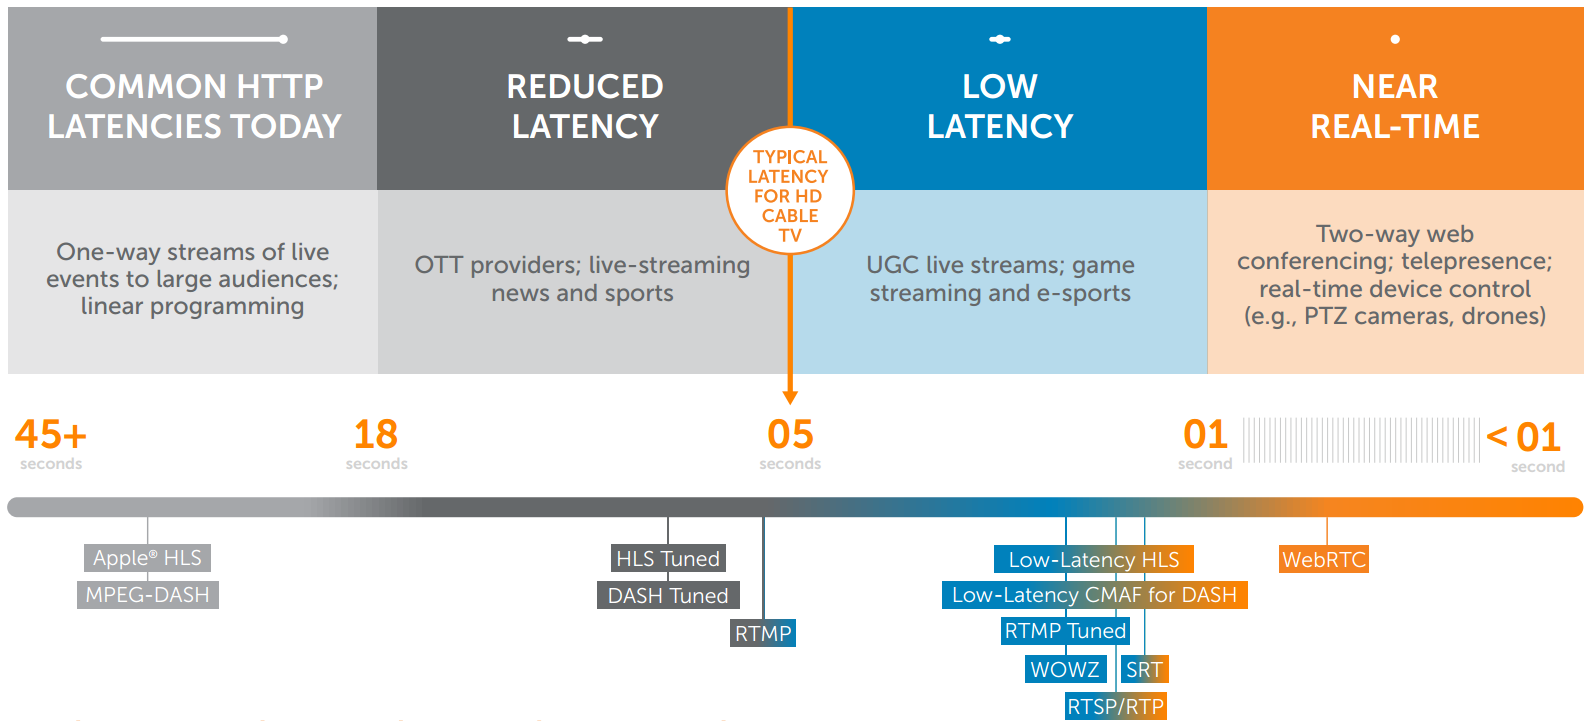
\includegraphics[width=0.99\linewidth]{protocol_latency.png}
	\caption{流媒体协议延迟及相关应用场景\cite{2019VideoStreaming2019}}
	\label{fig:protocol-latency}
\end{figure}

流媒体协议与封装格式的选择往往是相互关联的,一种流媒体协议可能会要求使用某种封装格式。下文会对不同流媒体协议进行对比,结合AV1相关的封装格式的情况,选择合适的流媒体协议。

\subsection{有状态流媒体协议}

有状态流媒体协议主要有RTMP、RTSP等,加上近年来比较热门的SRT协议。有状态流媒体协议通常底层使用UDP协议,因而延迟较低,但伸缩性较差。

\paragraph{RTMP} Real Time Messaging Protocol(实时消息传输协议)是Adobe的专有协议,旨在互联网上传输音视频数据。RTMP是基于TCP的协议,可维护持久连接并允许低延迟通信。为了平稳地传递流并传输尽可能多的信息,它将流分成多个片段,并在客户端和服务器之间动态协商其大小。由于以下原因等,RTMP难以应对当今的挑战:

\begin{enumerate} [label=\arabic*)]
    \item RTMP是Adobe的专有协议,Adobe暂停了对FLV与RTMP标准的更新;
    \item RTMP一般传输的是FLV格式,而FLV格式对编码标准有限制,只支持到H.264,不支持HEVC和AV1等较新的编码标准;
    \item RTMP无法优雅地支持高分辨率以及VR,360视频等,因为缺乏对新的编码标准的支持,以及由于带宽限制,RTMP无法以高比特率使用;
    \item RTMP遇到安全性,多语言支持和广告插入支持方面的问题;
    \item CDN厂商对RTMP的支持正在减弱,转而使用HLS和MPEG-DASH。
\end{enumerate}

\paragraph{RTSP} 实时流协议(Real Time Streaming Protocol, RTSP)由IETF标准化,在1998年以RFC2326\cite{schulzrinneRealTimeStreaming1998}的形式发布,RTSP2.0在2016年以RFC7826\cite{schulzrinneRealTimeStreamingProtocol2016}的形式发布,以替代RTSP1.0。RTSP是一种网络控制协议,专为娱乐和通信系统的使用,以控制流媒体服务器。流数据本身的传输不是RTSP的任务,大多数RTSP服务器使用实时传输协议(RTP\cite{schulzrinneRTPTransportProtocol2003})和实时控制协议(RTCP)进行媒体流传递。RTSP对编码标准的支持性取决于音视频编码标准的RTP封装协议支持,而一般的音视频编码标准都有相对应的RTP封装协议支持。

RTSP一般用于IP摄像头,也可以用于流媒体直播,其一大优势是延迟较小。RTSP的一大缺点是设备支持性差,在Android和iOS设备上没有开箱即用的RTSP兼容播放器,RTSP在web端的支持性也不好。

\paragraph{SRT} 实时可靠传输协议(Secure Reliable Transport, SRT)由Haivision和Wowza共同创建,并于2017开源。SRT通过动态适应传输端点之间的实时网络状况,优化了跨不可预测的网络(例如Internet)的流传输性能。这有助于最小化抖动和带宽变化的影响,而纠错机制有助于最大程度地减少数据包丢失。SRT旨在解决视频在公共互联网(网络质量不好)的分发挑战。SRT协议是和编码标准无关的,其传输的格式为MPEG-TS封装,因此需要音视频编码标准能够支持MPEG-TS封装协议。SRT在底层使用UDT协议,在此基础上做了拥塞控制策略的相关优化以降低传输延时。SRT协议也有一些缺陷,包括协议复杂度较高,丢包场景下速度退避较大等。一般将SRT用于视频上行到转码服务器。

\paragraph{WebRTC} WebRTC是一个免费的开源项目,通过简单的API为Web浏览器和移动应用程序提供实时通信(RTC)。WebRTC为视频会议设计,可以达到百毫秒级延迟,但同时因为这个设计初衷,WebRTC的伸缩性很差,难以用作直播用途。WebRTC正在通过W3C和IETF进行标准化。

\subsection{基于HTTP的自适应流媒体协议}

基于HTTP的自适应流媒体协议的基本思想是生成相同内容的多个版本(不同分辨率及码率),并将视频切分成数秒时长的片段,通过一个描述文件来整合片段信息。并且,与基于RTP的协议不同,基于HTTP的自适应流媒体协议可以穿越允许标准HTTP流量通过的任何防火墙或代理服务器。这允许从常规HTTP服务器提供内容,并通过广泛使用的基于HTTP的内容传递网络(CDN)传递内容,因此,基于HTTP的自适应流媒体协议有着较好的伸缩性。现在主流的基于HTTP自适应流媒体协议是苹果公司的HLS和MPEG-DASH。

\paragraph{HLS} HTTP实时流媒体协议(HTTP Live Streaming)是Apple开发并于2009年发布的基于HTTP的自适应比特率流通信协议,并由IETF标准化为RFC8216\cite{pantosHTTPLiveStreaming2017}。该协议的支持在媒体播放器,Web浏览器,移动设备和流媒体服务器中得到了广泛的应用。HLS的延迟一般在十秒级。iOS设备只能使用HLS协议。通过使用LHLS可以提供更低的延迟,主要优化了切片策略、播放列表策略等实现。

%TODO \cite dash? iso/iec的
\paragraph{MPEG-DASH} Dynamic Adaptive Streaming over HTTP(MPEG-DASH)是第一个国际标准的基于HTTP的自适应比特率流解决方案。与类似但更为专有的解决方案(例如Microsoft的Smooth Streaming或Adobe的HDS)相比,对自适应流解决方案进行标准化意味着要向市场提供该解决方案可用于通用部署的信心。与HDS或MSS不同,DASH与编解码器无关,这意味着它可以使用以任何编码格式编码的内容,例如H.265,H.264,VP9等,当然也可以使用AV1编码格式的内容。

\paragraph{CMAF} Common Media Application Format(CMAF)是一个标准化的容器,它的提出是为了解决流媒体行业中繁多的容器格式带来的问题,创建标准化的传输容器,以避免视频流工作流程中增加的成本与复杂性。。 随着流媒体协议的不同,文件容器也随之不同。HLS指定使用.ts格式Version7及以上可以使用fmp4格式,而DASH几乎统一使用基于ISOBMFF的.mp4容器。任何想要在Apple设备和Android设备上都吸引用户的内容分发者,必须对相同的音频和视频数据进行两次编码和存储,并且,相同内容、不同格式之间可能发生竞争,造成资源的浪费。

CMAF寻求的不仅仅是减少复杂性,除此以外,通过分块编码和分块传输编码,CMAF可以改善延迟,这将补充基于HTTP的自适应流媒体协议在实时交付上的能力,CMAF可以提供低于3秒的延迟。

\subsection{AV1的封装协议}

AV1的支持封装协议有Matroska/WebM、ISOBMFF、RTP,AV1没有官方支持的MPEG-TS封装协议。

% https://www.matroska.org/technical/specs/index.html
\paragraph{Matroska} Matroska是一个自由,开放标准的多媒体容器格式,可以在一个文件中数量不受限制地存放视频,音频,图片或字幕轨道。Matroska的核心设计特性主要有文件内的快速查找;高错误恢复率;分章节;可选字幕;可选音频轨;模块化的可扩展性;基于互联网的流传输;类似DVD提供的菜单。AV1的Matroska/WebM封装在开放标准Matroska中有相应的规范\cite{AOMAV1Codec}。

\paragraph{WebM} WebM是一种专为Web设计的开放,免版税的媒体文件格式。WebM的文件结构基于Matroska容器。WebM的针对网络传输进行了优化,致力于满足在网络上提供视频的独特需求:低计算量,设备适应性好、容器格式简单、高质量的实时视频交付等。WebM项目主要由Google团队开发,支持的视频编码标准有VP8、VP9、AV1等。

%https://aomediacodec.github.io/av1-isobmff/
\paragraph{ISOBMFF} ISO/IEC基本媒体文件格式(ISO/IEC Base Media File Format)定义了基于时间的多媒体文件的通用结构。ISOBMFF用作其他容器格式的基础,如MP4以及CMAF等。ISOBMFF定义于ISO/IEC 14496-12\cite{InformationTechnologyCoding},AOMedia推出了AV1视频编码的ISOBMFF协议规范\cite{concolatoAV1CodecISO}。

%https://aomediacodec.github.io/av1-rtp-spec/
\paragraph{RTP} 实时传输协议(Real-time Transport Protocol, RTP)是一种用于在IP网络上传输音视频的网络协议。RTP设计在UDP上运行,为抖动补偿,数据包丢失和无序传送的检测提供了便利。RTP通常与RTCP结合使用。RTP是由Internet工程任务组(IETF)的音频视频传输工作组开发的,最早于1996年作为RFC1889\cite{audio-videotransportworkinggroupRTPTransportProtocol1996}发布,然后于2003年被RFC3550\cite{schulzrinneRTPTransportProtocol2003}取代。对于各音视频编码的RTP封装支持,一般都有对应的RFC协议定义其分包、合包逻辑。AOMedia推出了AV1视频编码的RTP封装草案\cite{RTPPayloadFormat},尚未提交IETF标准化。

\paragraph{MPEG-TS} MPEG传输流(MPEG Transport Stream, MPEG-TS 或 TS)是用于传输和存储音频,视频以及节目和系统信息协议数据的标准数字容器格式。用于DVB,ATSC和IPTV等广播系统。MPEG传输流是为不太可靠的传输(即地面或卫星广播)而设计的,具有纠错和同步模式功能,可在承载该流的通信信道降级时保持传输完整性。MPEG-TS在ISO/IEC 13818-1\cite{InformationTechnologyGeneric}中定义。MPEG-TS将每个流切分成最多188个字节的部分,可以以更少的延迟和更大的容错性来交错流,但与此同时,MPEG-TS较小的切分方式会带来更多的额外开销。AOMedia未官方推出AV1的MPEG-TS封装协议,这可能是因为MPEG-TS是为广播设计的传输协议,本身不适合在互联网上传播。

% \subsection{传输协议与封装协议的关联与选择限制}


\subsection{AV1低延迟直播系统的传输与封装协议选择}

因为在章节\ref{sec:codec-comparison}中选择了AV1编码标准作为直播系统的编码,在直播系统的传输与封装协议选择时,有两个选择标准:1. 必须是AV1编码标准支持的;2. 尽量满足低延迟的互联网传输。基于这两点,由表\ref{tab:protocol}有以下分析:

\begin{enumerate} [label=\arabic*)]
  \item 对于基于HTTP的自适应流媒体传输协议,HLS对封装格式的需求是MPEG-TS或fmp4,前者AV1没有官方的协议支持,后者包含在对ISOBMFF的支持中,可以实现;对于DASH,AV1支持使用WebM封装或fmp4封装。但基于HTTP的自适应流媒体传输协议的延迟一般较高;
  \item 对于RTMP协议,不支持AV1编码协议,不予考虑;
  \item 对于RTSP协议,AV1支持其所需的RTP封装格式,在延迟上性能较好;
  \item 对于SRT协议,AV1并没有MPEG-TS封装协议支持,但SRT可以用作上行到转码服务器的传输协议;
  \item 对于WebRTC,虽然它有着最优秀的延迟性能,但是由于其设计是面向视频会议,伸缩性较差,不适合作为热流直播的协议选择。
\end{enumerate}

综上,综合考虑支持性和延迟、伸缩性(Scalability,指通过简单的增加硬件配置而使服务处理能力呈线性增长的能力),选择RTSP作为AV1低延迟直播系统原型的传输协议。

% 加入LHLS / CMAF?
\begin{table}[!hpt]
  \caption{AV1的传输与封装协议分析}
  \label{tab:protocol}
  \centering
  \begin{tabular}{cccc} \toprule
    协议     & 封装格式       & 延迟     & 伸缩性\\ \midrule
    HLS     & MPEG-TS, fmp4 & 10-45s  & good  \\
    DASH    & WebM, fmp4    & 10-45s  & good  \\
    RTMP    & /             & 5s      & normal \\
    RTSP    & RTP           & 2s      & normal \\
    SRT     & MPEG-TS       & 2s      & normal \\
    WebRTC  & RTP           & <1s     & bad    \\ \bottomrule
  \end{tabular} \\ \raggedright \vspace{8pt} \qquad \qquad \qquad \qquad
	\small 注:表中为典型应用场景下的协议延迟。
\end{table}



% \section{FFmpeg}

\section{本章小结}

本章是本论文研究需要涉及的基础知识,简要介绍了视频编码与视频编码标准的基础概念、AV1编码标准的编码工具,特别是其多层预测框架,介绍了AV1码流封装成“开放比特流单元(OBU)”的方式;介绍了常用的流媒体传输协议,其中包括有状态协议和基于HTTP的自适应流媒体协议,以及常见的多媒体封装协议,并根据相关协议的特性,结合对AV1编码标准的支持性与低延迟的要求,最终为直播系统原型构建选择了RTP作为封装格式,RTSP作为传输协议,选择SRT作为上行传输协议。